%!TEX root = ../thesis_a4.tex

\chapter{Introduction}
\label{sec:intro}

\section{Motivation}
\label{sec:intro:motivation}

We are witnessing an unprecedented information explosion thanks to the dramatic technological advancement brought by the Information Age \citep{smith2009social}. This technological (r)evolution has enabled the release and publication of huge amounts of data into online repositories such as web sites, forums, wikis, and social media. Art and culture have benefited dramatically from this context, which allows potentially anyone with an available Internet connection to access, produce, publish, comment, or interact with any form of media. 

In this context, music content creation, publication and dissemination has changed dramatically. Online music services, such as Pandora, Spotify, Apple Music, Google Play, Deezer, Tidal, Amazon Music, or Soundcloud, benefit from this situation and currently offer ever-growing catalogs with dozens of millions of music tracks, which are in turn just one click away from millions of users. This vast availability of music poses two serious challenges: First, \textit{how can a musical item be properly annotated and classified within a large collection?} Since manually managing these large libraries is not feasible due to size constraints, automatic methods for the annotation and classification of large-scale music collections have been an active area of research in recent years \citep{Schedl2014}. Second, \textit{how can a user explore or discover preferred music from all the available content?} Traditionally, users have relied on their friends, their favorite music radio host, a music expert in their local retail store, etc. to obtain recommendations on artists or albums they might like. Although this traditional approach is still valid and used by many people, its ability to cover the vast amount of available music nowadays is seriously hindered. Therefore, automatic approaches to music recommendation have become necessary \citep{celma2008new}.

Large music collections combine information from multiple data modalities, such as audio, images, text or videos. In addition, music collections can be enriched with user generated content published online. However, most of this content is still unusable by machines due to the fact that it is mostly created by humans and for humans, and hence it only exists in human readable form. In this context, Natural Language Processing plays a key role, as one of its main lines of research is precisely to transform human readable content into machine readable data \citep{cowie1996information}. %Allowing discovery of new facts and trends hidden in, for example, music libraries, blogs, web sites, journals or social networks.

The way human readable content and multimodal data present in large music collections is represented and combined in computational models poses numerous challenges. Artificial intelligence methods, such as machine learning, heavily rely on the choice of data representation. Therefore, finding representations that maximize the different explanatory factors of variation behind the data is a fundamental task. Traditional approaches rely on handcrafted features to represent the variability of the data, whereas more recently, and thanks the raise of deep learning techniques, representation learning approaches have demonstrated their superiority in multiple domains \citep{bengio2013representation}.

In this thesis, we address the aforementioned challenges of classification and recommendation of musical items in large music collections from two different stand points: (1) extracting structured knowledge from music-related texts and further enriching this knowledge with semantic information present in online knowledge repositories, (2) learning new data representations from heterogeneous data using deep learning architectures and further combining these representations in multimodal networks. %Both ideas are in turn applied to the aforementioned problems of classification and recommendation of musical items.
We hypothesize that such enriched knwoledge and learned multimodal data representations are crucial for improving recommendation and classification algorithms. %disrupting traditional approaches in different directions.
%we aim to advance the field of Music Information Retrieval. 

\section{Applied methodologies}

This thesis is framed within the Music Information Retrieval (MIR) research tradition. 
MIR is a multidisciplinary field of research concerned with the extraction, analysis, and usage of information about any kind of music entity (e.g. song, artist, album) on any representation level (e.g. audio signal, symbolic MIDI, metadata) \citep{schedl2008}. According to \cite{Schedl2013}, the musical factors that influence human music perception can be categorized into \textit{music content} and \textit{music context}.%, \textit{user context} and \textit{user properties}. 
Music context relates to all musical aspects that are not encoded in the audio signal, such as song lyrics, artist's biography, album cover artwork, or music video clips, whereas music content is defined as human perceptual aspects that can be extracted from the audio signal. %User context is related to the activity, mood or spatio-temporal aspects of the user when listening to music, and user properties to her music preferences, education or demographics. 
Following this distinction, research methodologies within the MIR community that deal with data modalities different from audio (e.g. text, images) are often called context-based approaches, whereas methodologies based on the analysis of the audio signal are called content-based approaches. 
Although we agree with this classification criteria, in this dissertation we follow the nomenclature used in the Recommender Systems community \citep{Ostuni2013} and consider \textit{audio signal}, \textit{text} (e.g. metadata, artist's biographies, song lyrics), and \textit{images} (e.g. album cover artwork, artist's photographies)as different modalities of content.

\subsection{Why knowledge extraction?}
\label{sec:intro:nlp}

As pointed out by \cite{humphrey2012}, MIR approaches are typically based on a two-stage architecture of feature extraction and semantic interpretation, e.g., classification, regression, clustering, similarity ranking, etc. 
Traditionally, MIR has been mainly focused on the use of features extracted from audio, and has not paid much attention to other data modalities. However, in recent years several studies have shown the benefits of using context-based and multimodal approaches \citep{Schedl2014}. 

Audio features are often classified into low, mid and high-level representations \citep{bello2005}. Low-level representations (e.g. \textit{spectral flux, cepstrum, MFCCs}) are measured directly on the audio signal. Mid-level representations (e.g. chords, onsets) represent musical attributes extracted from the audio combining machine learning and musical knowledge. High-level representations (e.g. mood, form, genre) are related to human interpretations of the data, and are typically built on top of low and mid-level representations. The extraction and exploitation of features from these three representation levels have been widely studied in the MIR field. 

Following this feature hierarchy, when dealing with textual data, we can also differentiate between low, mid, and high-level representations. Low-level representations (e.g. word frequencies, word co-occurrences, n-grams) are measured directly on text. Mid-level representations (e.g. part-of-speech tags, named entities) combine linguistic knowledge and statistical analysis of text corpora. High-level representations (e.g. syntactic dependencies, semantic relations) involves a semantic understanding of text. In the context of MIR, most of the literature is focused on low-level representations, few in mid-level, and almost none in high-level. Little attention has been paid to the semantic of words or in the context they are being used. Thus, the research in the MIR field, has not yet exploited the epistemic potential of text.

In the first part of this thesis, we focus on text-based approaches. On the one hand, we work on new methodologies for the extraction of high level semantic representations from unstructured texts. On the other hand, we put the emphasis on the development of approaches that exploit these semantic representations in MIR tasks, such as music recommendation and classification. In addition, we study how semantic information may impact musicological studies.

\subsection{Why multimodal deep learning?}
\label{sec:intro:learning}

As stated before, MIR approaches are commonly based on a two-stage architecture of feature extraction and semantic interpretation. In this context, data representations are generally obtained following a traditional feature extraction process, which involves a combination of music domain-knowledge, psychoacoustics, and audio engineering \citep{humphrey2012}. 
This is known as feature engineering, and compensates the inability of traditional machine learning algorithms to extract the discriminative information of the data. However, it involves a labor-intensive human effort, and also all the different explanatory factors of variation behind the data are not represented \citep{bengio2013representation}. 
Huge efforts have been put in the last two decades in the definition and extraction of audio features, which has given rise to comprehensive software libraries that assemble many of these feature extraction techniques \citep{bogdanov2013essentia, Mcfee2015}. 

Contrarily to feature engineering, representation learning (or feature learning) is a technique that allows a learning system to automatically discover the variation behind the data directly from raw signals. As shown by \cite{humphrey2012}, MIR approaches can benefit from the use of these learning approaches using deep neural networks. This methodology has two main advantages. First, blurring the boundaries between the two-stage architecture, which implies fully-automated optimization of both stages at once. Second, it results in general-purpose architectures that can be applied to different MIR problems and data modalities. In the last years, several works have been published where audio-based deep learning architectures have been applied to MIR tasks such as music recommendation \citep{Oord2013} and music classification \citep{Choi2016}, among others. However, to the best of our knowledge, there is no multimodal system that makes use of deep learning approaches for music recommendation or music classification.

While in the first part of the thesis we use data representations based on traditional feature engineering approaches, in the second part of this dissertation we focus on representation learning approaches using deep neural networks. We apply this methodology to different data modalities (audio, text and images) and their combination, and in the context of music recommendation and classification tasks.

\section{Challenges addressed}

%The main objective of this thesis is to improve the classification and recommendation of musical items in large music collections, with special emphasis on novel and less popular items. To do so, we have addressed two different approaches, one related to the extraction of structured knowledge from unstructured text sources, and the other related to the learning of new data represantations from multimodal data. However, while working in the former approach, we discovered that it may be also applied to other music related problems such as the automatic creation of music knowledge repositories or the discovery of musicological knowledge. %, which are more related to the understanding of music. 
%Therefore, in addition to classification and recommendation, we have also addressed these linguistic and musicological problems.
%In Figure\ref{fig:intro:chapters}, a diagram of this thesis is shown, organized according to the different approaches, methods, and applications present in each chapter. 
In this section we describe in detail the two main challenges addressed in this dissertation: music classification and music recommendation.

\subsection{Music classification}
\label{sec:intro:annotation}

The advent of large music collections has posed the challenge of how to access the information in terms of retrieval, browsing, and recommendation. One way to ease the access of large music collections is to keep annotations of all music resources \citep{sordo2012semantic}. Annotations can be added either manually or automatically. 
%Manual annotation of huge music collections is too costly due to high human effort required. 
However, due to the high human effort required for manual annotations, the implementation of automatic annotations processes has become a necessity. 

We distinguish two ways of automatically enhancing annotations: (i) gathering annotations from external sources, and (ii) learning annotations from the collection's data. To address (i), information can be obtained from online knowledge repositories (e.g. Wikipedia, MusicBrainz), or extracted from collections of unstructured documents. This imposes the challenge of how to properly map collection's items with external entities. To address (ii), machine learning techniques can be applied over the collection's data. When annotations are learned from audio, this classification task is often called auto-tagging. However, annotations can be learned from different data modalities, such as album cover artworks, tags, editorial metadata, video clips, etc.

Among the different categories of annotations used in music collections, the most prototypical are: music genres, instruments, and moods. 
Music genre labels are useful categories to organize and classify songs, albums and artists into broader groups that share similar musical characteristics. Music genres have been widely used for music classification, from physical music stores to streaming services. Automatic music genre classification thus is a widely explored topic \citep{sturm2012survey}.
However, almost all related work is concentrated in the classification of music items into broad genres (e.g., Pop, Rock), assigning a single label per item \citep{bogdanov2016cross}. This is problematic since there may be hundreds of more specific music genres \citep{pachet2000taxonomy}, and these may not be necessarily mutually exclusive (i.e., a song could be Pop, and at the same time have elements from Deep House and a Reggae groove). 

In this thesis, we focus on the problem of enriching annotations in music collections from the two above defined standpoints, i.e. gathering and learning. We study how semantic technologies may be useful to improve the annotations of musical items. In addition, we tackle the problem of multi-label music genre classification from different data modalities (i.e., audio, text, and images) and their combination.


\subsection{Music recommendation}
\label{sec:intro:recommendation}

Information overload in modern Web applications challenges users in their decision-making tasks. Recommender systems have emerged in the last years as fundamental tools in assisting users to find, in a personalized manner, what is relevant for them in overflowing knowledge spaces \cite{ricci2011introduction}. 

Music recommendation is a relatively young but continuously growing research topic, in both MIR and Recommender Systems communities. Although several research approaches and commercial systems have been proposed in the last decade, many of them are adaptations from other domains \citep{oscarBook}. 
Music has its own specificities with respect to other domains. For instance, a user may consume a musical item several times, or very different items according to the user context (e.g. working, dinning, exercising). Therefore, music recommendation is a challenging and still unsolved problem.

\begin{figure}
	\centering
	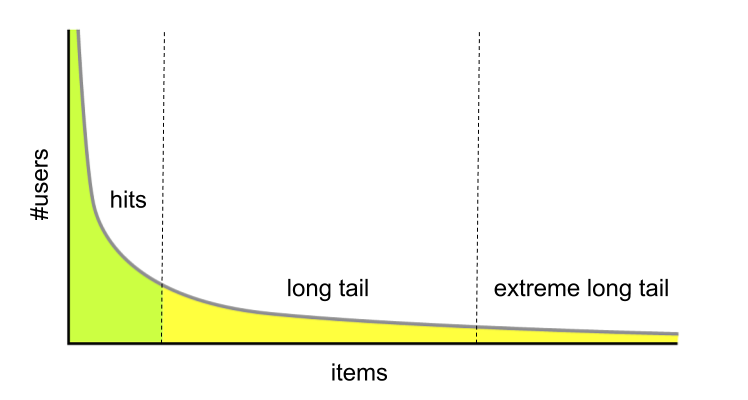
\includegraphics[width=0.7\textwidth]{ch01_intro_pics/Long_tail.png}
	\caption{Long tail distribution.\label{fig:soa:longtail}}
\end{figure}

Although music online services make available almost all existing music, only a small percentage of these catalogs is actually consumed by the vast majority of users. Music consumption follows what is called a \textit{long tail} distribution \citep{oscarBook} (see Figure~\ref{fig:soa:longtail}). Therefore, one of the main challenges in music recommendation is how to make this niche of unknown musical items profitable. Moreover, as new music is continuously being created, new artists and releases appear every day. Hence, another important challenge in music recommender systems is how to deal with these new items, which is often called the \textit{cold-start} problem. % TODO: Anadir algo mas sobre cold-start y diferencia con long tail

To tackle these problems, it is crucial to have good items descriptions and to exploit all the available multimodal data (e.g., images, audio, texts, and videos).
The web is full of user generated content with relevant information about music, which has the potential to impact in the performance of music recommender systems. However, as stated before, this content is mostly unstructured and requieres the application of knowledge extraction techniques that exploit the semantic of texts.
In addition, up to now, audio content has been barely exploited in commercial recommender systems. However, thanks to the advent of novel deep learning approaches that raised the accuracy of audio-based recommendations \citep{Oord2013}, audio may turn into a key factor in order to provide accurate long tail recommendations.

Most research in music recommendation has been dedicated to developing algorithms that provide \textit{good} and \textit{useful} recommendations~\citep{oscarBook}, neglecting the importance of the novelty and diversity of recommendations \citep{adomavicius2012improving,Bellogin2010}. In addition, very few approaches are able to provide explanations of the recommendations to the users~\citep{Passant2008, Passant2010}. According to~\cite{celma2008new}, giving explanations of the recommendations provides transparency to the recommendation process and increases the confidence of the user in the system.

In this thesis we further explore into the music recommendation problem from three different perspectives. First, we investigate how information extracted from large collections of music-related documents may be useful to provide explanations of recommendations to users. Second, we tackle the problem of recommending long tail items by leveraging semantic information from knowledge repositories and combining that with users feedback data. Finally, we address the problem of cold-start music recommendations by combining different data modalities using deep neural networks.


\section{Objectives and outline of the thesis}
\label{sec:intro:objectives}

\begin{figure}
	\centering
	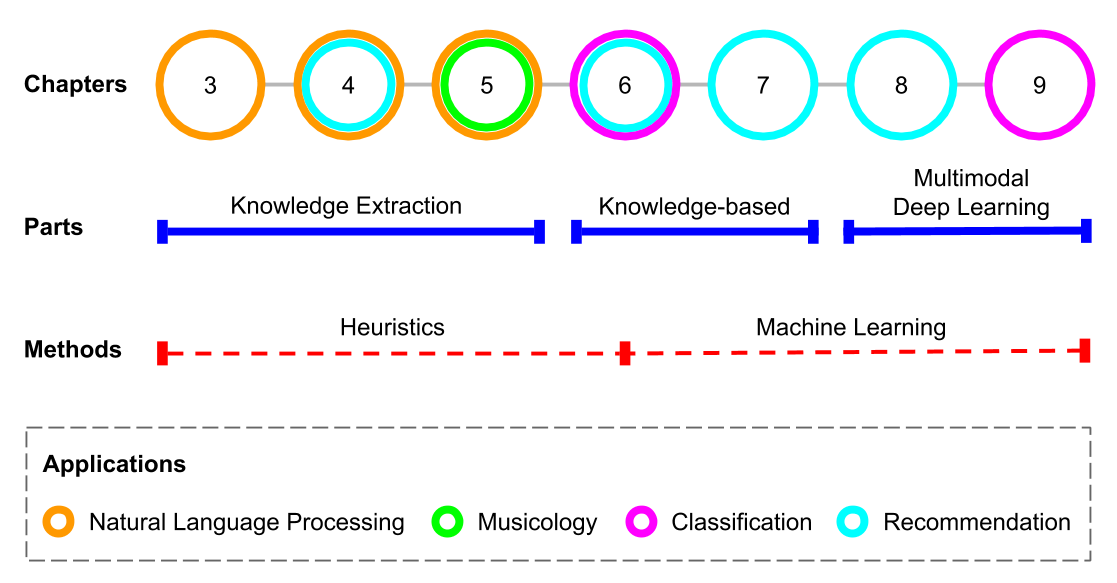
\includegraphics[width=\textwidth]{ch01_introduction_pics/Thesis_schema.png}
	\caption{Thesis overview.\label{fig:intro:chapters}}
\end{figure}

In the previous sections we have explained the motivations and context of our thesis. According to that, the main objective of this dissertation is to improve the classification and recommendation of musical items in large music collections, with special emphasis on the promotion of novel and less popular items. To do so, we have addressed two different methodologies, one related to the extraction of structured knowledge from unstructured text sources and its further enrichment using information present in online knowledge repositories, and the other related to the learning of new data represantations from multimodal data using deep learning architectures. The former approach may be also applied to other music related problems such as the creation of music knowledge repositories or the discovery of musicological knowledge. %, which are more related to the understanding of music. 
Therefore, in addition to the classification and recommendation problems, we have also addressed these linguistic and musicological challenges.
In Figure\ref{fig:intro:chapters}, a diagram of this thesis is shown, organized according to the different approaches, methods, and applications present in each chapter. Although this thesis is focused on the music domain, we strongly believe that the work we present can be easily adapted to other multimedia domains. 


%In the previous sections we have explained the motivations and context of our thesis. According to that, the main goal of this dissertation is to push the state of the art in music recommendation and classification by leveraging knowledge repositories and unstructured text sources, and learning novel data representations from multimodal data using deep neural networks. Although this thesis is focused on the music domain, the work we present can be easily adapted to other multimedia domains. Figure\ref{fig:intro:chapters} shows a conceptual organization of the chapters of this thesis according to the different approaches, methods, and applications.

This thesis is structured as follows: Chapter~\ref{sec:SOA} presents some background knowledge and related work on Natural Language Processing, Recommender Systems, and MIR. Hereafter, the work in this dissertation is divided in two Parts: In Part~\ref{part:knowledge-extraction} we explore different techniques and approaches to extract semantic information from unstructured music-related text sources. Then, these semantic representations are exploited in Music Classification, Similarity and Recommendation problems. Within this Part, Chapter~\ref{sec:linking} illustrates the problem of linking musical texts and knowledge repositories. In Chapter~\ref{sec:kb} we address the automatic generation of Music Knowledge Bases from unstructured text sources. This Chapter encloses with an experiment on explanations of music recommendations based on extracted knowledge. In Chapter~\ref{sec:musicology}, three experiments study the potential impact of knowledge extraction techniques in musicological studies.
Chapter~\ref{sec:similarity} presents the application of a semantic-based approach to music similarity and classification problems, whereas Chapter~\ref{sec:graph-rec} addresses the problem of long tail recommendations by enriching annotations with semantic information.
Then, in Part~\ref{part:multimodal-deep} an approach to learn data representations from different data modalities using deep neural networks is applied to the Music Recommendation and Classification problems. In Chapter~\ref{sec:cold-rec} we address the problem of cold-start music recommendations using audio and text. Finally, in Chapter~\ref{sec:multi-class} we apply a similar approach for multi-label classification of music gernes using audio, text, and images.
At the end of each chapter, we include a focused discussion about the relevant results and conclusions. We conclude this thesis in Chapter~\ref{sec:conclusion} with a summary of our work, our main conclusions, and a discussion about open issues and future perspectives.




